% !TeX root = ../main.tex
\chapter{基于SVM的股票价格预测模型}

\section{整体思路}

与前人所做的工作不同,本文采取量化K线的策略,研究的对象为具有特定形态组合的股票数据,以此作为基础来训练SVM回归模型。

实现基于SVM的股票价格预测模型的思路是:首先选择对股价预测有重要参考价值的指标;再提取与之相对应的历史数据;
并从中筛选出具有特定形态组合的数据;然后对数据进行预处理和标准化;根据数据特征选择SVM核函数;
在每一个不同的$T$上,将清洗后的数据作为训练样本输入模型;利用超参数寻优方法寻找最佳超参数;
最后得到最终模型,利用测试样本检验模型的准确性。

\section{处理步骤}

模型的具体实现流程如下:

\subsection{确定指标}

股票市场是一个高度复杂的非线性系统,受到多种因素的影响,因此所选择的指标必须充分反映股票市场的交易特征。
指标体系必须满足实用性原则和灵活性原则,尽可能得简化并且易于获取,并能够充分描述股票市场。
由于本文对日线与周线分别做了分析,于是我们所选择的基础指标如表(3.1)。
\begin{table}[ht]
    \centering
    \caption{选择的数值指标}
    \begin{tabular}{lcc}
        \hline
        {指标名称} & {日线指标含义} & {周线指标含义}\\
        \hline
        {Open\underline{~~}up} & {昨日开盘价} & {上周开盘价}\\
        {Close\underline{~~}up} & {昨日收盘价} & {上周收盘价}\\
        {High\underline{~~}up} & {昨日最高价} & {上周最高价}\\
        {Low\underline{~~}up} & {昨日最低价} & {上周最低价}\\
        {Vol\underline{~~}up} & {昨日成交量} & {上周成交量}\\
        {Amount\underline{~~}up} & {昨日成交金额} & {上周成交金额}\\
        {Open\underline{~~}down} & {今日开盘价} & {这周开盘价}\\
        {Close\underline{~~}down} & {今日收盘价} & {这周收盘价}\\
        {High\underline{~~}down} & {今日最高价} & {这周最高价}\\
        {Low\underline{~~}down} & {今日最低价} & {这周最低价}\\
        {Vol\underline{~~}down} & {今日成交量} & {这周成交量}\\
        {Amount\underline{~~}down} & {今日成交金额} & {这周成交金额}\\
        {T\underline{~~}mean} & {未来$T$个交易日平均最低价} & {未来$T$个交易周平均最低价}\\
        \hline
    \end{tabular}
\end{table}

\subsection{实验样本}

本文中,我们的目的是希望当某一只股票出现某种特定的模式的时候,通过SVM模型来预测未来$T$个交易周期的最低价平均值,来为投资者提供投资建议。

\subsubsection{实验对象}

本文选取了中国大陆市场上所有股票,收集其2016年01月04日至2019年08月15日之间的相关数据,即开盘价、收盘价、最高价、最低价、成交量与成交金额。
根据投资周期划分,可以将投资者的行为分为短期投资和长期投资,于是本文不仅收集了日线的数据,也收集了周线和月线的数据。
但由于月线数据进行进一步筛选后数据量过少,没有实验意义,遂舍弃。
本文仅根据上述收集的日线与周线数据进行预测分析,
接着我们在日线上将数据筛选出2种特定的数据组合:
\begin{enumerate}
    \item 日线\underline{~~}1,今日成交量大于昨日成交量,且今日收盘价大于昨日收盘价。
    \item 日线\underline{~~}2,今日成交量大于昨日成交量,且今日收盘价大于昨日收盘价,且今日最低价小于昨日最低价。
\end{enumerate}

两种数据形态组合分别如图(3.1)和图(3.2)所示。

\begin{figure}[ht]
    \centering
    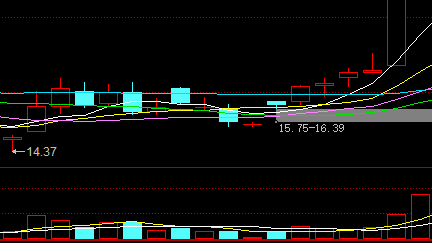
\includegraphics[scale=1]{case 1.png}
    \caption{第一种数据形态组合的例子}
\end{figure}

\begin{figure}[ht]
    \centering
    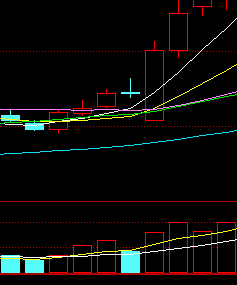
\includegraphics[scale=1]{case 2.png}
    \caption{第二种数据形态组合的例子}
\end{figure}

在周线上也将数据筛选成了2种特定的数据组合:
\begin{enumerate}
    \item 周线\underline{~~}1,这周成交量大于上周成交量,且这周收盘价大于上周收盘价。
    \item 周线\underline{~~}2,这周成交量大于上周成交量,且这周收盘价大于上周收盘价,且这周最低价小于上周最低价。
\end{enumerate}
然后再通过时间序列统计方法计算了未来$T$个交易日/周的平均最低价,其中我们计算了$T=2\sim15$总计14个交易周期的平均最低价。
其中,获取到的部分数据如表(3.2),以日线\underline{~~}1,$T=15$为例。

\begin{table}[ht]
    \centering
    \caption{日线\underline{~~}1,$T=15$}
    \resizebox{\textwidth}{12mm}{
    \begin{tabular}{lllllllllllll}
        \hline
        Open\underline{~~}up &  Close\underline{~~}up &  High\underline{~~}up &  Low\underline{~~}up &     Vol\underline{~~}up &     Amount\underline{~~}up &  Open\underline{~~}down &  Close\underline{~~}down &  High\underline{~~}down &  Low\underline{~~}down &   Vol\underline{~~}down &   Amount\underline{~~}down &     T\underline{~~}mean \\
        \hline
            9.03 &      9.17 &     9.17 &    9.01 &  1013673.0 &  9.681270e+08 &       9.24 &        9.18 &       9.33 &      9.15 &  1279688.0 &  1.240686e+09 &   8.948667 \\
           13.88 &     13.91 &    14.09 &   13.73 &  2444548.0 &  3.479176e+09 &      14.04 &       13.94 &      14.51 &     13.91 &  2656294.0 &  3.849312e+09 &  13.630667 \\
           12.29 &     12.32 &    12.50 &   12.16 &  1013663.0 &  1.278185e+09 &      12.48 &       12.34 &      12.56 &     12.16 &  1045757.0 &  1.318960e+09 &  11.583333 \\
            8.58 &      8.63 &     8.74 &    8.49 &   638272.0 &  5.595231e+08 &       8.73 &        8.66 &       8.79 &      8.63 &   649476.0 &  5.766833e+08 &   9.594000 \\
           12.15 &     12.17 &    12.34 &   11.90 &  1157650.0 &  1.416000e+09 &      12.34 &       12.21 &      12.49 &     12.09 &  1411794.0 &  1.757797e+09 &  12.252000 \\
        \hline
    \end{tabular}}
\end{table}

至此必要的原始数据全部收集完毕,可以进行进一步处理。

\subsubsection{样本规模}

样本的规模很容易会影响到SVM的性能和核函数的选择,
如果样本规模太大,由于SVM算法涉及到凸优化,其算法的时间复杂度是$O(n^2)$的,将会导致训练时间过长,影响超参数优化的速度;
如果样本规模太小,则会影响SVM回归预测的准确性。

本文对上述数据统计整理后,结果如表(3.3)。
\begin{table}[ht]
    \centering
    \caption{样本的规模,单位:个}
    \begin{tabular}{lcccc}
        \hline
        {$T$} & {日线\underline{~~}1} & {日线\underline{~~}2} & {周线\underline{~~}1} & {周线\underline{~~}2}\\
        \hline
        {$T=2$} & {24017} & {1301} & {3243} & {184}\\
        {$T=3$} & {23124} & {1275} & {3151} & {177}\\
        {$T=4$} & {22557} & {1233} & {2949} & {164}\\
        {$T=5$} & {21952} & {1186} & {2851} & {158}\\
        {$T=6$} & {21433} & {1154} & {2779} & {154}\\
        {$T=7$} & {20442} & {1081} & {2660} & {150}\\
        {$T=8$} & {19885} & {1042} & {2592} & {149}\\
        {$T=9$} & {19455} & {1004} & {2267} & {139}\\
        {$T=10$} & {18752} & {973} & {2217} & {136}\\
        {$T=11$} & {18210} & {930} & {2128} & {131}\\
        {$T=12$} & {17508} & {857} & {2060} & {125}\\
        {$T=13$} & {16689} & {833} & {1941} & {122}\\
        {$T=14$} & {16182} & {807} & {1867} & {117}\\
        {$T=15$} & {15636} & {767} & {1795} & {116}\\
        \hline
    \end{tabular}
\end{table}
显而易见的是,样本的规模随着$T$的增加而逐渐减少,这是由数据本身的性质决定的,
因为我们是根据未来$T$个交易周期来计算最低价平均值,当无法获取到特定时间的最低价时,计算便会被终止并舍弃该数据。
另外可以看到,日线\underline{~~}1的样本数据量最大,训练时间最长,拟合预测的效果最好。
本文将这些样本按$4:1$的比例随机分成2组:一组作为训练样本,用于模型构建与优化;一组作为测试样本,用于检验模型的预测效果。

\subsection{数据预处理}

\subsubsection{异常值处理}

前面提到,SVM所生成的超平面依赖于支持向量,但如果这些支持向量中包含异常点,将会对整个模型的性能产生影响。
所以我们需要在数据预处理时清除数据的异常点,在本文中我们利用Tukey's Test来粗略地检测异常值。其原理如下:
\begin{enumerate}
    \item 将数据从小到大排列,计算下四分位数$Q_1$,和上四分位数$Q_3$。
    \item 用公式估计出数据的最大值$MAX=Q_1-t(Q_3-Q_1)$和最小值$MIN=Q_3+t(Q_3-Q_1)$。
    \item 当数值$X<MIN$或$X>MAX$时,被认为是异常值,予以去除,其他的为正常值。
\end{enumerate}

其中的$t$值经过多次实验后确定为$1.3$,能够较好的保持样本规模的条件下去除异常值。
异常点处理完毕后,进入下一流程:数据标准化。

\subsubsection{数据标准化}

数据的标准化(Normalization)是对数据进行缩放,使之落入一个小的区间。
标准化对SVM来说有2个好处:一是避免特征之间量级差异过大造成不平衡;而是提高模型收敛,即求最优解的速度。
数据标准化的常用方法有$Min\text{-}Max$标准化和$Z\text{-}score$标准化。

$Min\text{-}Max$标准化将数据线性变换到$[0,1]$区间内,转换函数为:
\begin{align}
    x^*=\frac{x-x_{min}}{x_{max}-x_{min}}
\end{align}
其中$x_{max}$和$x_{min}$分别为原始数据的最大值和最小值,$x^*$和$x$分别为转换后的数据和原始数据。

$Z\text{-}score$标准化利用原始数据的均值$\mu$和标准差$\sigma$进行标准化,因此又称标准差标准化,经过处理的数据符合标准正态分布。
转换函数为:
\begin{align}
    x^*=\frac{x-\mu}{\sigma}
\end{align}
其中$\mu=\frac{1}{n}\sum_{i=1}^nx_i$,$\sigma=\sqrt{\frac{1}{n-1}\sum_{i=1}^n(x_i-\mu)^2}$。

本文中,通过多次测试,最终选用表现更好的$Z\text{-}score$标准化来进行数据标准化处理。

\subsection{核函数选择}

根据前人的经验和实验的反复检验,我们将选择使用RBF核函数,理由如下:
\begin{itemize}
    \item 线性核函数是RBF核函数的一个特例,使用RBF核函数则无需考虑线性核函数。
    \item 多项式核函数有2个参数$\gamma$和$d$,而RBF核函数只有1个参数$\gamma$,参数越多则模型越复杂,训练时间就越长,超参数寻优时也更耗时。
    \item 本次实验的样本数量不算大也不算小,RBF核函数的性能更有优势。
\end{itemize}

\subsection{超参数寻优}

选取RBF核作为SVM的核函数后,我们需要优化两个超参数,一个是RBF核的参数$\gamma$,另一个是惩罚系数$C$。
两个参数决定了SVM回归模型的学习能力和泛化能力,我们可以认为模型产生了一个以$\gamma$和$C$为自变量的黑盒函数$Score=F(\gamma,C)$,
令人遗憾的是没有任何办法获取黑盒函数的具体形态,于是超参数寻优便成了当前一个很重要的研究问题,
目前随着自动机器学习框架的研究和发展,目前已经萌生出许多种超参数优化方法:

\subsubsection{交叉验证法}

先手动选择参数,然后交叉验证法将训练数据分成2个部分,用其中较大的部分构建模型,用较小的部分检验模型计算误差。
多折交叉验证则是将数据分成多个部分,并将每个部分作为较小的部分来检验根据其余部分的组合所构建的模型,再计算每折交叉验证的平均误差来作为评判标准。
但是反复地选择参数费时费力,不适合多参数的寻优问题。

\subsubsection{网格搜索法}

网格搜索的基本思想是,手动选择多个$\gamma$与多个$C$使其组合成多个参数组,作为搜索空间,
然后对所有参数组合计算预测误差,最终选择出误差最小的参数组合。
通过这种方法基本上可以找到全局最优解,能够避免重大误差的出现。
但是,对于参数搜索空间太大的情况,网格搜索的效率是极其低下的,而且我们并没有办法一次性确定好初始的参数搜索空间。

\subsubsection{随机搜索法}

随机搜索与网格搜索的区别只在第一步:随机搜索从参数空间中随机选取参数组合。
通过随机搜索我们可以更广泛地搜索超参数空间,虽然不一定能找到全局最优点,
但我们可以用更少的迭代次数来寻找较优的参数组合,这是在提高寻参速度和降低预测误差之间的一种权衡方式。

网格搜索和随机搜索的每一次寻优计算都是相互独立的,没有利用先验知识来选择下一组超参数。

\subsubsection{进化算法}

进化算法在各个领域都得到了不错的应用,其主要特点是直接对结构对象,即参数组合进行操作,并采用概率化的寻优方法,
能够自适应地调整搜索方向,自动获取搜索空间。其主要流程是,先对参数组合进行编码,初始化种群,
评估个体的适应度,再通过选择、交叉和变异等手段来保留最佳的个体(例如,改动其中一个超参数)。

\subsubsection{粒子群算法}

粒子群算法通过设计一种无质量和体积的粒子来模拟鸟群,仅有速度和位置两种属性。
每个粒子在搜索空间中单独地寻找最优解,然后将个体最优解与其他粒子共享,每个粒子再根据个体最优解和全体最优解来调整自己的速度和位置,
即通过个体的优化来实现群体的优化。

进化算法与粒子群算法的缺陷在于,算法容易陷入局部最优值。

\subsubsection{基于顺序模型的全局优化算法}

基于顺序模型的全局优化(Sequential Model-Based Optimization,SMBO)算法已经用于许多应用中,
其首先在多个参数组合中收集先验知识,即预测误差,然后进行一些推断并确定接下来要尝试的参数组合。
SMBO算法使用代理函数来逼近真正的黑盒函数,内部优化算法是对代理函数的迭代和优化,目前主流的有:
\begin{enumerate}
    \item 贝叶斯优化:使用高斯过程对代理函数进行建模。
    \item 基于序列模型的算法配置(Sequential Model-based Algorithm Configuration,SMAC):基于SMBO,利用了使用过的结果好的模型(高斯随机过程模型),并引入了随机森林来处理分类参数。
    \item 树状结构Parzen估计方法(Tree-structured Parzen Estimator,TPE):是SMAC的改进版本,用两个分离的模型进行后验的模拟,进一步加快寻优速度。
\end{enumerate}

大量的实验表明,TPE算法优于随机搜索算法\cite{bergstra2011algorithms},
另外,由于计算资源有限,本文将使用交叉验证与TPE算法相结合来进行超参数寻优。

\subsection{拟合预测}

将通过交叉验证与TPE算法超参数寻优得到的最优参数组合来构建SVM回归预测模型,使用此模型对测试数据进行检验,计算预测误差。

\subsection{误差评价}

本文仅选用均方误差$MSE$来对模型的预测效果进行评估,$MSE$是预测值和真实值之间差的平方和的期望,其计算方法如下:
\begin{align}
    MSE=\frac{1}{n}\sum_{i=1}^n(y_{pred}-y_{true})^2
\end{align}
$MSE$是评估数据变化程度的重要指标,较小的值则说明SVM回归预测模型所预测的数据有相当高的精确度。